\begin{figure}
	\centering
	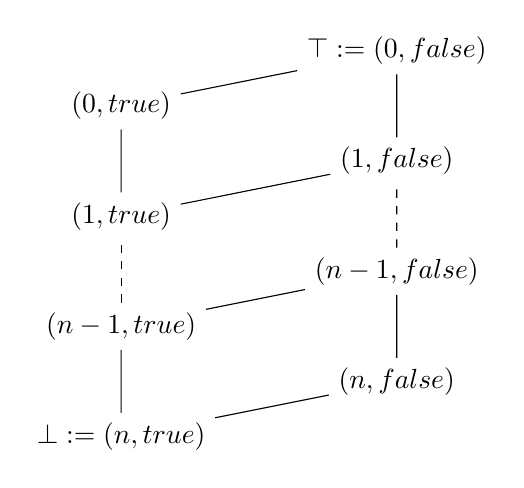
\begin{tikzpicture}[scale=.7]
		\node (np0) at(0,0) {$\bot := (n,true)$};
		\node (np1) at(0,2) {$(n-1,true)$};
		\node (np2) at(0,4) {$(1,true)$};
		\node (np3) at(0,6) {$(0,true)$};
		\node (p0) at(5,1) {$(n,false)$};
		\node (p1) at(5,3) {$(n-1,false)$};
		\node (p2) at(5,5) {$(1,false)$};
		\node (p3) at(5,7) {$\top := (0,false)$};
		\draw (np0) -- (p0) -- (p1) -- (np1) -- (np0);
		\draw (np2) -- (p2) -- (p3) -- (np3) -- (np2);
		\draw [dashed] (np1) -- (np2);
		\draw [dashed] (p1) -- (p2);
	\end{tikzpicture}
\caption{Hesse diagram of the lattice which is used in this analysis}
\label{fig:lattice}
\end{figure}